\documentclass{article}
\usepackage[utf8]{inputenc}
\usepackage[margin=1in]{geometry}
\usepackage{graphicx}

\title{Machine Learning Algorithms Overview}
\author{Hanchung Lee}
\date{February 2020}

\begin{document}

\maketitle

\section{Lasso Regression}

\noindent
\begin{enumerate}
    \item \textbf{What are the basic concepts? What problem does it solve?}
    \noindent 
    \smallbreak
    Lasso regression is an extension of basic regression with an \verb|L1 norm| regularization term $\mathbf{\lambda}\left\| \mathbf{W}\right\|_{1}$ where $\mathbf{\lambda}$ is a coefficient vector that adjusts the regularization of individual parameters $\mathbf{W_{i}}$. \cite{1} The $\mathbf{\lambda}$ term is also called the \emph{shrinkage}
    
    In other words, Lasso is similar to Ridge where both helps adding biases to the model to improve the out of the sample fit of the model.
    Lasso is especially useful for dealing with sparse data.

    \item \textbf{What are the assumptions?}
    \noindent 
    \smallbreak
    The same as regression, assuming \verb|i.i.d.| of sampled data.
    
    \item \textbf{What are the steps of the algorithm?}
    \noindent 
    \smallbreak
    Same as regression except adding an L1 norm term to penalize Weight coefficients of some variables. 
    
    Cross validation is used to select the regularization hyperparameter $\mathbf{\lambda}$.
    
    \item \textbf{What is the cost function?}
    \noindent 
    \smallbreak
    $$\mathbf{W}^{lasso} = {argmin}_\mathbf{W}} \left\{\frac{1}{2} \sum_{i = 1}^{N} (y_i - \mathbf{W}_0 - \sum_{j=1}^{P} x_{ij}\mathbf{W}_{j})^2 + \mathbf{\lambda}\sum_{j=1}^{P}\left\|\mathbf{W}_{i}\right\|_{1}\right\}$$ \cite{1}, where the first term within the $argmin$ is the mean squared error and the second term is the Lasso regularization. This can be solved with convex optimization.
    
    \item \textbf{Whare are the advantages/disadvantages?}
    \noindent 
    \smallbreak
    The prime difference between Lasso (L1) vs Ridge (L2) regularization of regression is that Lasso has the capability of forcing coefficients to $0$, and in effect, zeros out an feature variable. In essence, Lasso regression is doing feature selection.
    
    In a geometric sense, in high dimeisions, L1 norm will have many sharped edges and corners. During convex optimization, if the optimization hits the edges or corners, the coefficient become zero.  ON the other hand, L2 norm is a smooth surface thus it won't hit exactly model
    
    Thus, we can say that Lasso Regression yields a \emph{sparse} model where only a subset of the variables is in play. 
    
    Ridge is more suited for models with dense features while Lasso is more suited for models with sparse features. Use cross validation to determine the most suitable regularization.
    
    
\begin{figure}
  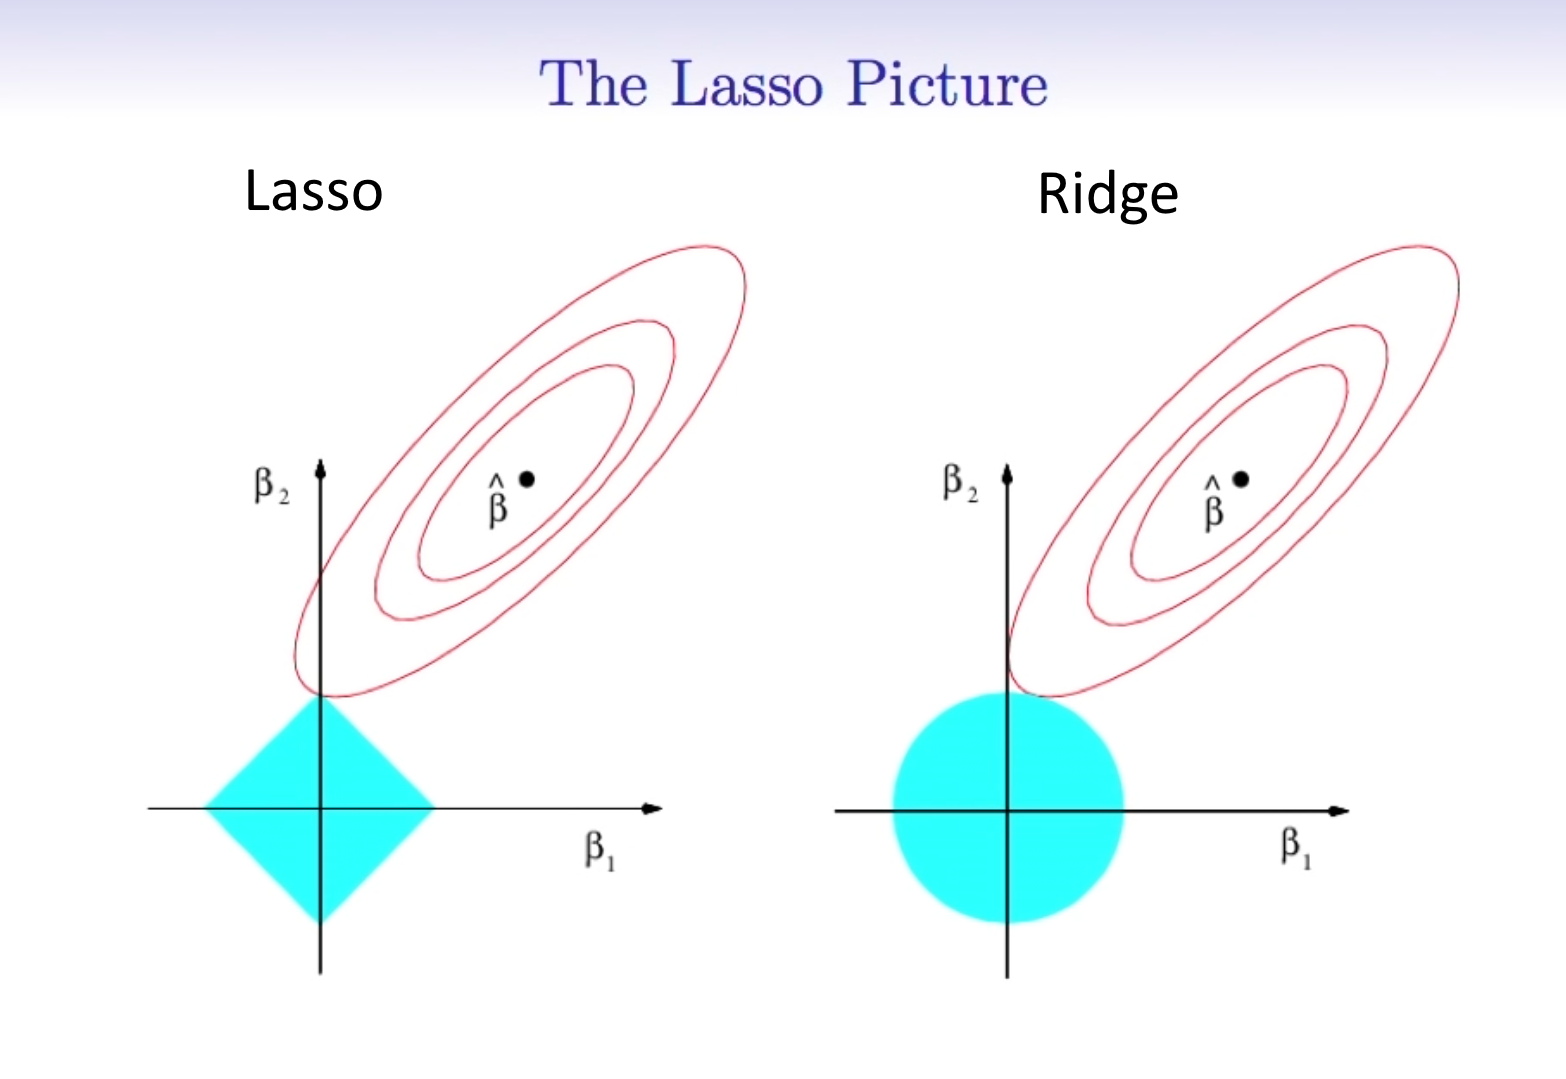
\includegraphics[width=\linewidth]{ridge_vs_lasso.png}
  \caption{Ridge vs Lasso}
  \label{fig:ridge_vs_lasso}
\end{figure}
    
\end{enumerate}

\section{Gradient Boosting}
\noindent
\begin{enumerate}
    \item \textbf{What are the basic concepts? What problem does it solve?}
    \noindent 
    \smallbreak
    Gradient boost decision tree models works by training many trees in sequence and ensemble the trees together at the end. When training sequentially, each of the newer trees are trained on the residual error observed by the previous tree. GBDT models tends to fit the training data well, with low bias and high variances. Because of that, it uses a learning rate $\lambda$ to scale contribution from a new tree. The idea is to take many small steps towards the right direction and ensemble them together result in a better prediction.

    \item \textbf{What are the assumptions?}
    \noindent 
    \smallbreak
    Decision tree based models makes no assumption about the distribution of the underlying data. In other words, decision trees are non-parametric.
    
    \item \textbf{What are the steps of the algorithm?}
    \noindent 
    \smallbreak
    Gradient boost initializes by building \verb|depth=1| node. It builds a tree depending on the depth and splits parameters. Then for the following trials it kept on building new trees to minimize the residual errors $(y - \gamma)$from the previous tree, and scale the contribution with a learning rate. The whole process is repeated $M$ times and the maximum depth of the individual trees is $J$.
    
    A formal definition is as follows \cite{1}
    \bigbreak
    \hline
    \noindent
    \textbf{Algorithm} Gradient Tree Boosting Algorithm
    \begin{enumerate}
    \hline
        \item Initialize $f_o(x) = argmin_{\gamma} \sum_{i=1}^{N} L(y_i, \gamma)$
        \item For \emph{m} = 1 to \emph{M}:
            \begin{enumerate}
                
                \item For \emph{i} = 1, 2, . . . , \emph{N} compute the pseudo residual term
                $r_{im} = -\left[ \frac{\partial L(y_i, f(x_i))}{\partial f(x_i)}\right]_{f = f_{m-1}}$
                \item For a regresion tree to the target $\emph{r}_{im}$ given terminal regions $R_{jm}, j = 1, 2, ..., J_m$
                \item For $j = 1, 2, ..., J_m$, find the new predicted value $\gamma$ \\
                $\gamma_{jm} = argmin_{\gamma} \displaystyle\sum_{x_i \in R_{jm}} L(y_i, f_{m-1}(x_i) + \gamma)$
                \item Update $f_m(x) = f_{m-1}(x) + \sum_{j=1}^{J_m} \gamma_{jm} I(x \in R_{jm})$
            \end{enumerate}
        \item Output $\hat f(x) = f_M(x)$
    \end{enumerate}
    \hline
    
    \item \textbf{What is the cost function?}
    \noindent 
    \smallbreak
    Given the standard loss function setup, $L(f) = \sum_{i=1}^{N} L(y_i, f(x_i))$, proper loss function $L(f)$ can be used for different settings. A summary table is as follows \cite{1}:
    \begin{center}
      \begin{tabular}{ l | l | l }
        \hline
        Setting & Loss Function & $ \frac{-\partial L(y_i, f(x_i))}{\partial f(x_i)}$ \\ \hline
        Regression & $\frac{1}{2}[y_i - f(x_i)]^2$ & $y_i - f(x_i)$ \\ \hline
        Regression & $\left\||y_i - f(x_i)|\right\|$ & $sign[y_i - f(x_i)]$ \\ \hline
        Regression & Huber & y_i - f(x_i) for |y_i - f(x_i)| \leq \delta_m \\ 
         & & \delta_m sign[y_i- f(x_i)] for |y_i - f(x_i)| > \delta_m \\ 
         & & where \delta_m \eq \alpha th-quantile \{|y_i - f(x_i)|\} \\ \hline
        Classification & Multinominal Deviance & \emph{k}th component: $I(y_i \eq G_k) - p_k(x_i)$ \\
        \hline
      \end{tabular}
    \end{center}
    
    \item \textbf{Whare are the advantages/disadvantages?}
    \noindent 
    \smallbreak
    Gradient boost is very similar to AdaBoost. The key difference is that for Gradient Boost, it can have a tree size that is larger than a stomp (depth of 1). Because gradient boosting is a boosting model that ensembles sequentially trained models, it is a naturally a low bias model. However, the downside is to a low bias model is the variance can be high and has to be reduced by adding regularization. Also, because the model is trained sequentially, it is compute intensive to train.
    
\end{enumerate}

\section{Neural Networks}
\noindent
\begin{enumerate}
    \item \textbf{What are the basic concepts? What problem does it solve?}
    \noindent 
    \smallbreak
    According to the Universal Approximator Theorum, neural networks is an universal function approximator that can be used approximate any functions that map $X \rightarrow Y$. It can be used abstracts away some of the feature engineering steps in classical machine learning tasks. For example, instead of designing image filters, CNN learns the filters itself, or instead of tagging word semantic labels, RNNs learns the relationships between words.
    
    The most fundamental neural network layer is a linear layer where $f(\mathbf{X}) = \sum_{m=1}^{M} g_m(\mathbf{W_m}\intercal\mathbf{X})$, where the input values go through an affine transformation and scaled by an activation function $g_m$. Activation functions usually tend to scale the outputs to pseudo range bound, such as sigmoid and Tanh. 

    \item \textbf{What are the assumptions?}
    \noindent 
    \smallbreak
    The assumptions are highly dependent on the structure of neural networks. For example, some neural network architectures such as convolution neural networks or recurrent neural nets assumes that the underlying data are \emph{i.i.d} while some other architectures such as Bayesian neural networks or Graph neural nets could have different assumptions about the relationships between feature spaces.
    
    \item \textbf{What are the steps of the algorithm?}
    \noindent 
    \smallbreak
    Neural networks is predominant solved using stochastic gradient descent with an auto differentiation library. First, inputs are feeded forward through the network for an output $\hat y$, and apply the loss function. The algorithm then take the gradients of the loss function and back propagate the network to obtain the differences in parameters between target and output. The parameters are then updated with the differences. One small batch at a time.
    \bigbreak
    \hline
    \noindent
    \textbf{Algorithm} Stochastic gradient descent (SGD) update at training iteration k \cite{2}
    \hline
    \smallbreak
    \textbf{Require:} Learning rate $\epsilon_k$
    
    \textbf{Require:} Initial parameter $\theta$
    
    \qquad \textbf{while} stopping criterion not met \textbf{do}
    
    \qquad \qquad Sample a minibatch of \emph{m} examples from the training set $\{x^{(1)}, ..., x^{(m)}\}$ with corresponding targets $y^{(i)}$
    
    \qquad \qquad Compute gradent estimate: $\hat g \leftarrow + \frac{1}{m}\nabla_{\theta}\sum_{i} L(f(x^{i};\theta),y_{(i)})$
    
    \qquad \qquad Apply update: $\theta \leftarrow \theta - \epsisolon\hat g$
    
    \qquad \textbf{end while}
    \smallbreak
    \hline

    \item \textbf{What is the cost function?}
    \noindent 
    \smallbreak
    Neural networks is an flexible architecture thus different loss functions can be used for different tasks. Typical loss functions includes cross entropy and negative log likelihood for classification and mean absolute error (L1) and mean squared error (L2) for regressions.
    
    \item \textbf{Whare are the advantages/disadvantages?}
    \noindent 
    \smallbreak
    Rather than considering neural networks as a kind of model, it is closer to a highly customizable building blocks for machine learning models. Depends on the complexity of the network constructed, it can be capable of learning a large amount of information from data. At the same time it excels in learning implicit relationships. 
    
    However, it is an black box model that is quite difficult to interpret and usually has to rely on large data sets and large amount of compute power to train. It is also difficult to debug and fine tune.
    
\end{enumerate}

\begin{thebibliography}{}
\bibitem{1}
Hastie, Tibshirani, and Friedman,
\emph{The Elements of Statistical Learning}.
2nd Edition,
2009.

\bibitem{2}
Goodfellow, Bengio, Courville,
\emph{Deep Learning},
2016

\bibitem{3}
Nasirany, Thomas, Wei, and Yang,
\emph{A Comprehensive Guide to Machine Learning},
2018

\end{thebibliography}
\end{document}
